%
% Metriken
% Abschlussarbeit (Bachelor)
%
% Thema: Erstellung einer Browser Extension zur Usability Evaluierung von beliebigen Web-Applikationen über Heatmaps.
% Betreuer 1: Prof. Dr. Targo Pavlista
% Betreuer 2: Siamak Haschemi
%
% @author Christian Bromann <contact@christian-bromann.com>
%

\newglossaryentry{Fixationen}{name=Fixationen, description={Als Fixationen werden sogenannte \textit{Eye-Stops} (Augenanhaltepunkte) bezeichnet.}}

\section{Metriken und Analyse}
\label{metrics}

Usability ist keine Eigenschaft, die einfach abzulesen ist. Sie ist ebenfalls nicht exakt bestimmbar und lässt sich ebenfalls nicht in numerischen Werten ausdrücken. Um sie herauszufinden, gibt es zwei Möglichkeiten. Entweder man vertraut seinem eigenen Gefühl beim Benutzen der Software oder erstellt Tests und nutzt Metriken zur Auswertung der Ergebnisse. Die Intuition ist wichtig und kann im ersten Moment viel aussagen, bietet jedoch keine wirkliche Sicherheit, da sie lediglich die eigene Meinung repräsentiert. Da eine Software von verschiedenen Personen mit unterschiedlichen Ansprüchen benutzt wird, reicht eine wage Vermutung nicht aus.\\
\\
Eine Usability-Studie bringt ein allgemeineres Abbild der Benutzbarkeit. Die aus den Tests erzeugten Daten lassen sich durch verschiedenste Metriken analysieren und auswerten. Sie unterliegen dabei keinen Richtlinien und spezialisieren sich teilweise auf bestimmte Aspekte bei der Benutzung einer Software. Abhängig davon, welche Aspekte analysiert und welche Daten dabei aufgezeichnet werden, erfolgt die Erstellung von Metriken ganz individuell für jeden Test. Sie bilden das Maß der Benutzbarkeit und sollten objektiv bestimmbar und vergleichbar sein.\\
\\
Usability-Tests lassen sich besser vergleichen, wenn Probanden Aufgaben während der Nutzung erledigen müssen. Metriken können dazu die Kriterien bieten. So kann bspw. verglichen werden, wie viele User eine bestimmte Aufgabe erfolgreich gelöst haben, wie lange sie dafür brauchten, wie viele Fehlermeldungen gezeigt wurden oder wie Zufrieden der User mit der Nutzung war. Hier reichen laut Nielsen \cite{metrics} schon 5 Personen aus, um einen aussagekräftigen Vergleich zu bekommen. Durch eine Gewichtung der Metriken oder der einzelnen Resultate kann sich der Test auf bestimmte Faktoren der Usability konzentrieren. So ist die Performance in manchen Situationen wichtiger als das Aussehen einer Seite. Bei der Auswahl der Testpersonen kann ebenfalls eine Gewichtung oder Einschränkung vorgenommen werden, wenn die Software lediglich für eine bestimmte Benutzergruppe bestimmt ist.\\
\\
Neben Metriken sind vor allem Aufmerksamkeits- und Aktivitätsverteilungen eine wichtige Methode zur Analyse der Usability. Diese stammen ursprünglich aus dem Eye-Tracking Verfahren und dienen dort vor allem zum Test der Wirksamkeit verschiedener Objekte und Elemente einer Software. Das Ergebnis der Verteilung kann auf verschiedenster Art und Weise visuell dargestellt werden. Zur Markierung der besonders aktiven Bereiche wird oft rot verwendet. Um so mehr die Aktivität abnimmt, um so kälter wird die Farbe. Zur Bestimmung der Aufmerksamkeit wird beim Eye-Tracking Verfahren die Bewegung der Pupille aufgezeichnet, um daraus den Focus des Auges möglichst genau zu bestimmen. Da dieses Verfahren recht aufwendig und teuer ist, kann im Bereich des Web-Usability-Testing auch auf die Mausposition zurückgegriffen werden. Da viele User die Maus benutzen, um Bereiche auf einer Internetseite zu entdecken, erzeugt dieses Mittel ebenfalls ein aussagekräftes Ergebnis.


\subsection{Clickmaps}

Die Aufmerksamkeit oder Aktivität eines Users kann durch verschiedene Faktoren bestimmt werden. Bei der Clickmap konzentriert sich dies auf jeden Klick, die der User auf der Seite tätigt, sei es in der Navigation oder auf einen Link im Text. Als ein Overlay über den Screenshot einer Seite zeigt es ziemlich genau an, wohin der User geklickt hat. Dabei stellt sich oft heraus, dass Elemente angeklickt werden, die lediglich von grafischer Bedeutung sind. Benutzer missinterpretieren häufig Bilder als Links zu anderen Seiten. Durch Clickmaps kann dieses Problem sehr leicht erkannt werden.

\vspace{0.3cm}
\begin{center}
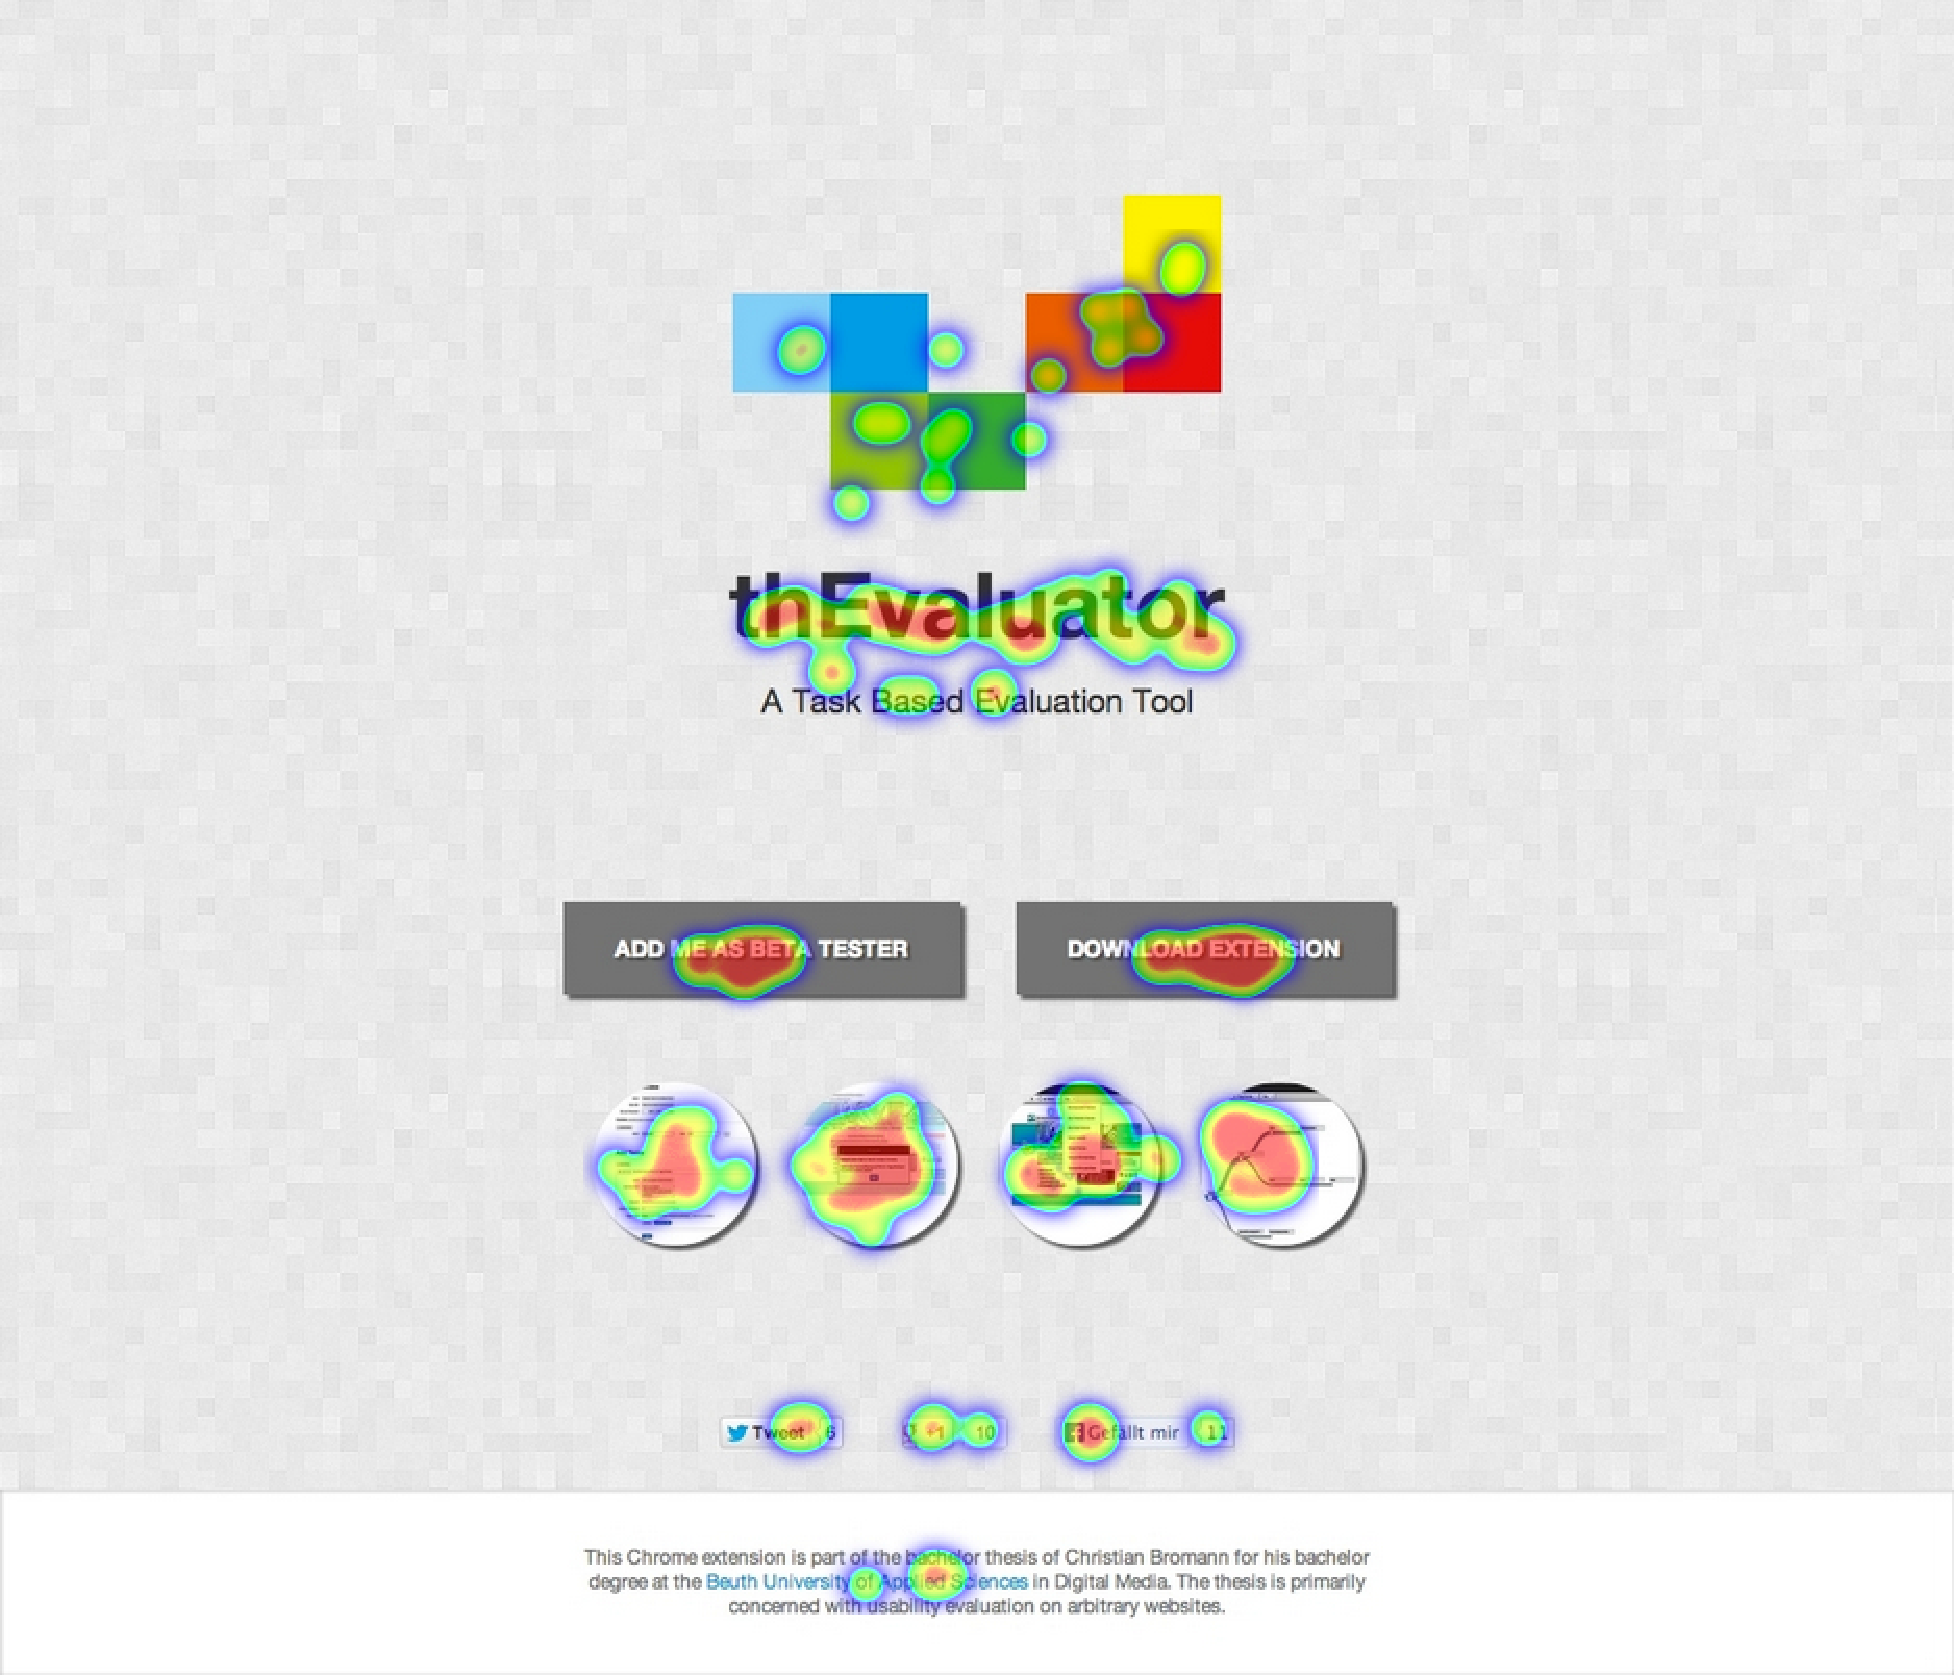
\includegraphics[scale=0.35]{./images/clickmap}
\end{center}
\begin{figure}[htb]
   \centering
   \caption{Beispiel einer Clickmap der \textit{thEvaluator} Projektwebsite}
    \label{clickmap}
\end{figure}


\subsection{Heatmap}

Bei Heatmaps bestimmt ein anderer Faktor die Aufmerksamkeit und Aktivität eines Benutzers. Hier wird neben dem Klickverhalten auch noch die $ x $ und $ y $ Position der Maus mit in die Berechnung der Heatmap mit einbezogen. Dadurch lassen sich große Datenwerte vereinfacht und anschaulich darstellen. Es ist teilweise sogar möglich, die Bewegung der Maus genau mitzuverfolgen. In Abbildung \ref{heatmap} werden die gleichen Daten verwendet, die bereits für die Abbildung \ref{clickmap} benutzt wurden. Hier lassen sich eindeutige Mausbewegungen verfolgen. Der Focus der Aufmerksamkeit dieser Seite ist klar erkennbar.

\vspace{0.3cm}
\begin{center}
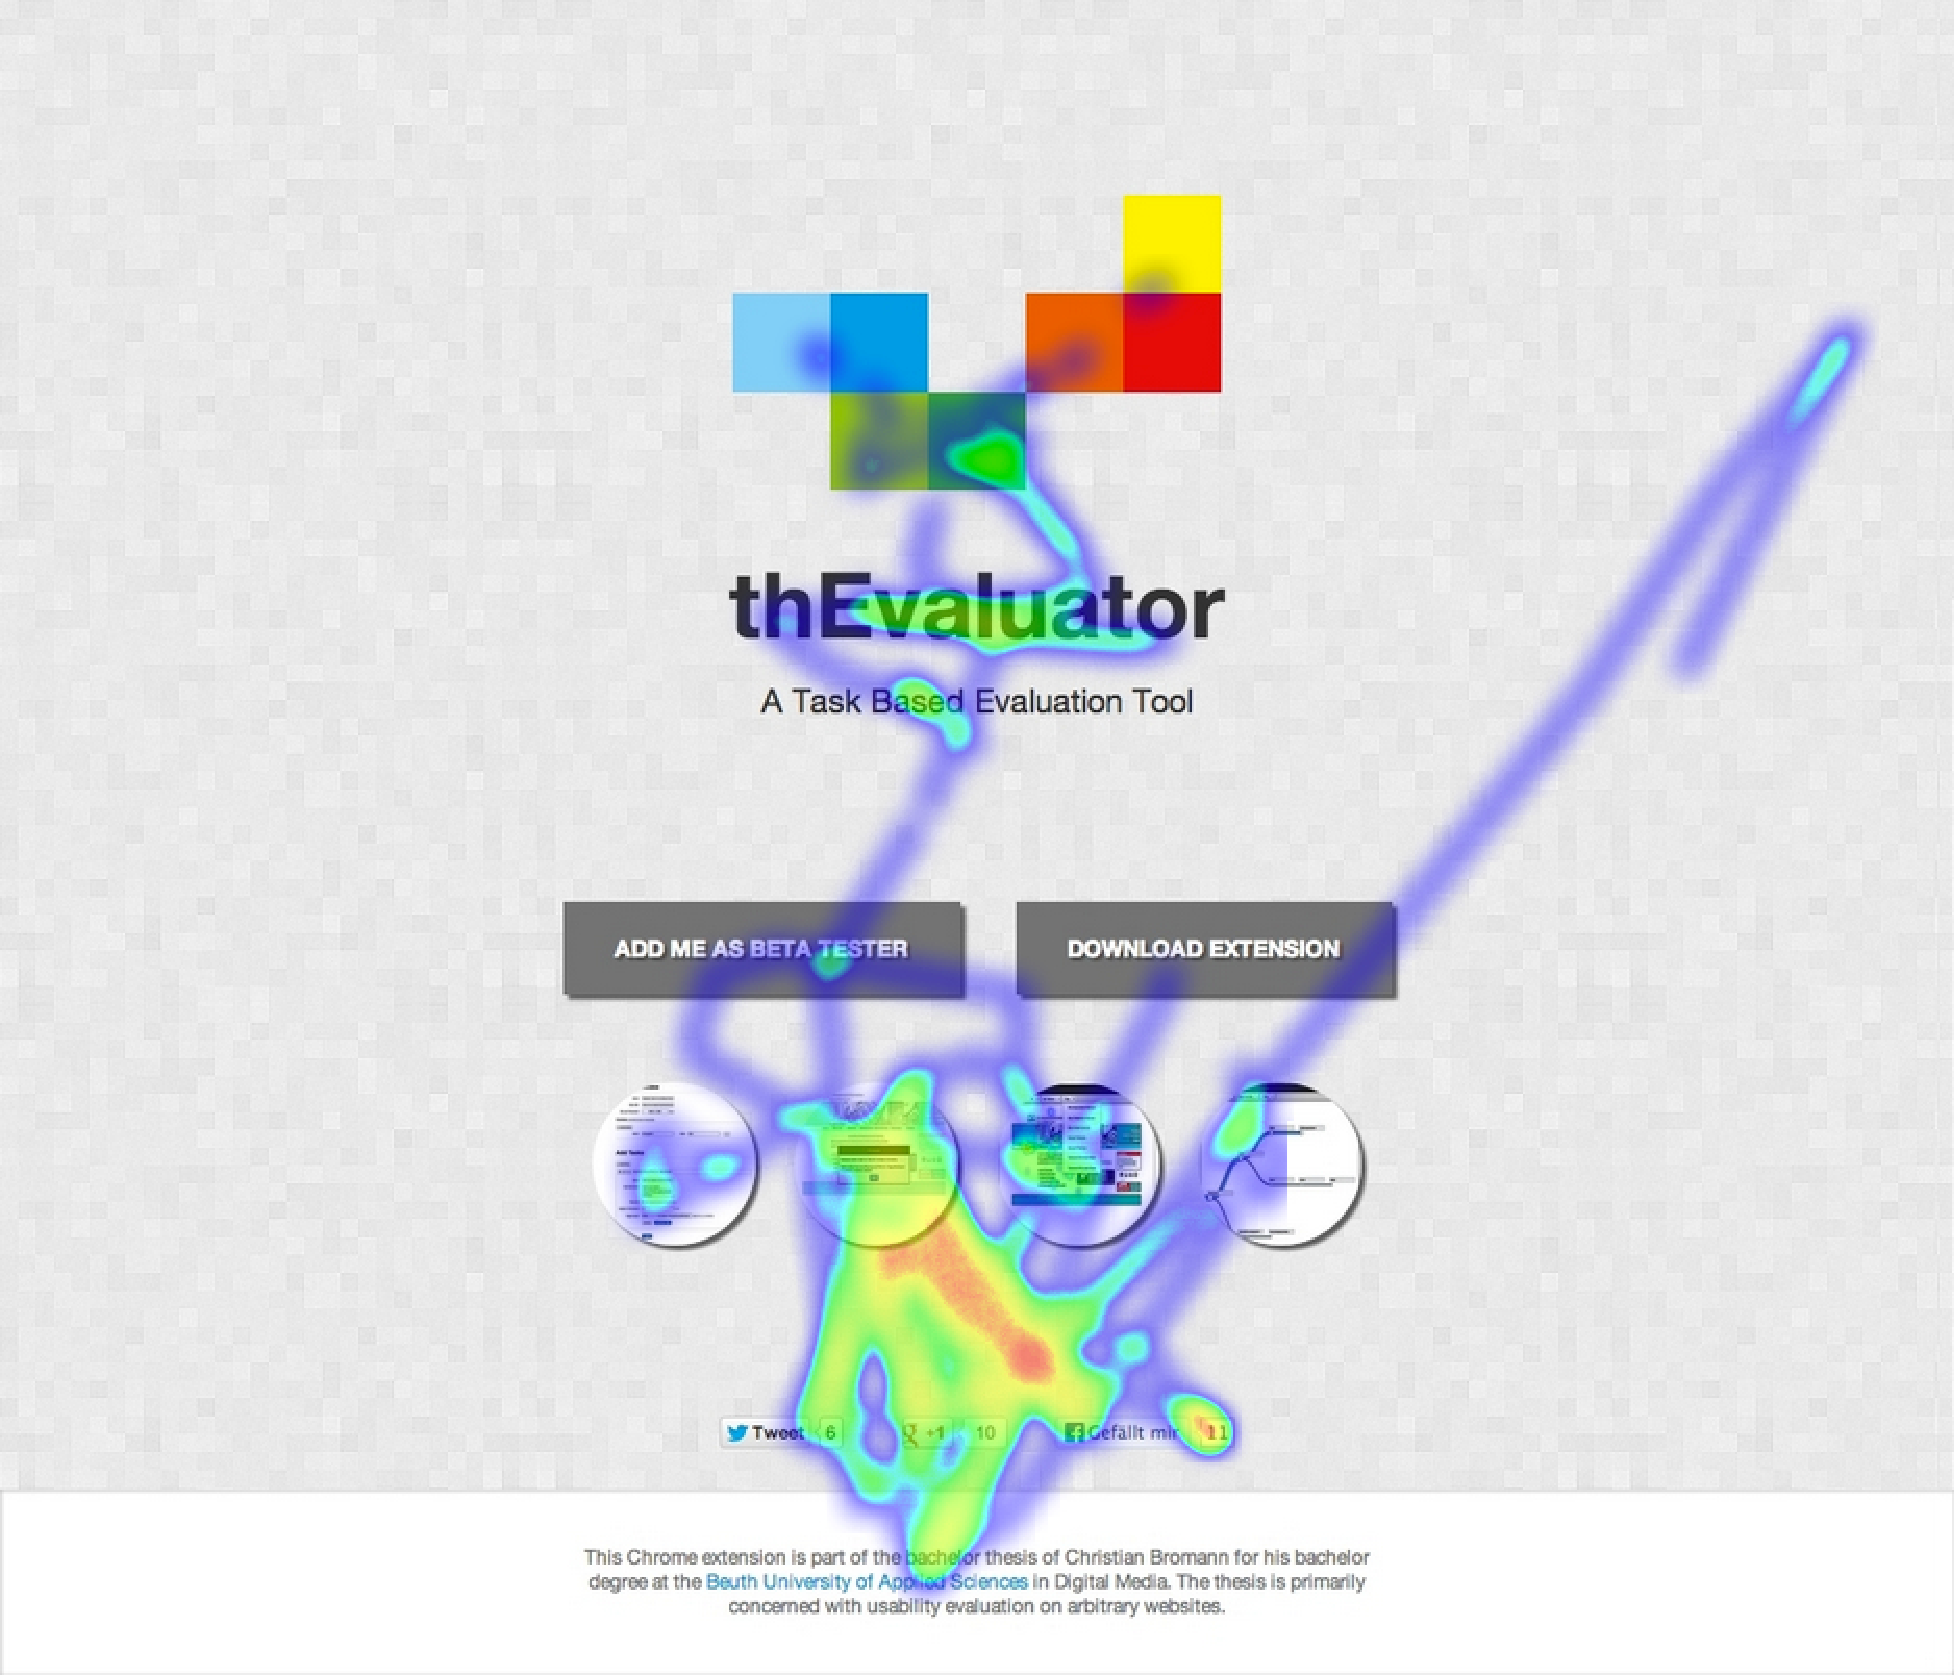
\includegraphics[scale=0.35]{./images/heatmap}
\end{center}
\begin{figure}[htb]
   \centering
   \caption{Beispiel einer Heatmap der \textit{thEvaluator} Projektwebsite}
    \label{heatmap}
\end{figure}


\subsection{Gazespots}

Aktivität kann auch durch Stillstand ausgedrückt werden. Betrachtet der Nutzer einen Punkt auf der Website intensiv, indem die Maus sich kaum dabei von der aktuellen Position fortbewegt, so kann man dies als Fixierung dieses Bereiches interpretieren und damit als Aufmerksamkeitsbereich. Je höher also die Betrachtungszeit eines Bereiches auf der Website ist, desto wärmer ist die Farbe auf dem Screenshot. Abbildung \ref{gazespot} zeigt, ebenfalls mit den gleichen Daten wie bei den letzten Abbildungen, die Fixierungspunkte der Projektwebsite.

\vspace{0.3cm}
\begin{center}
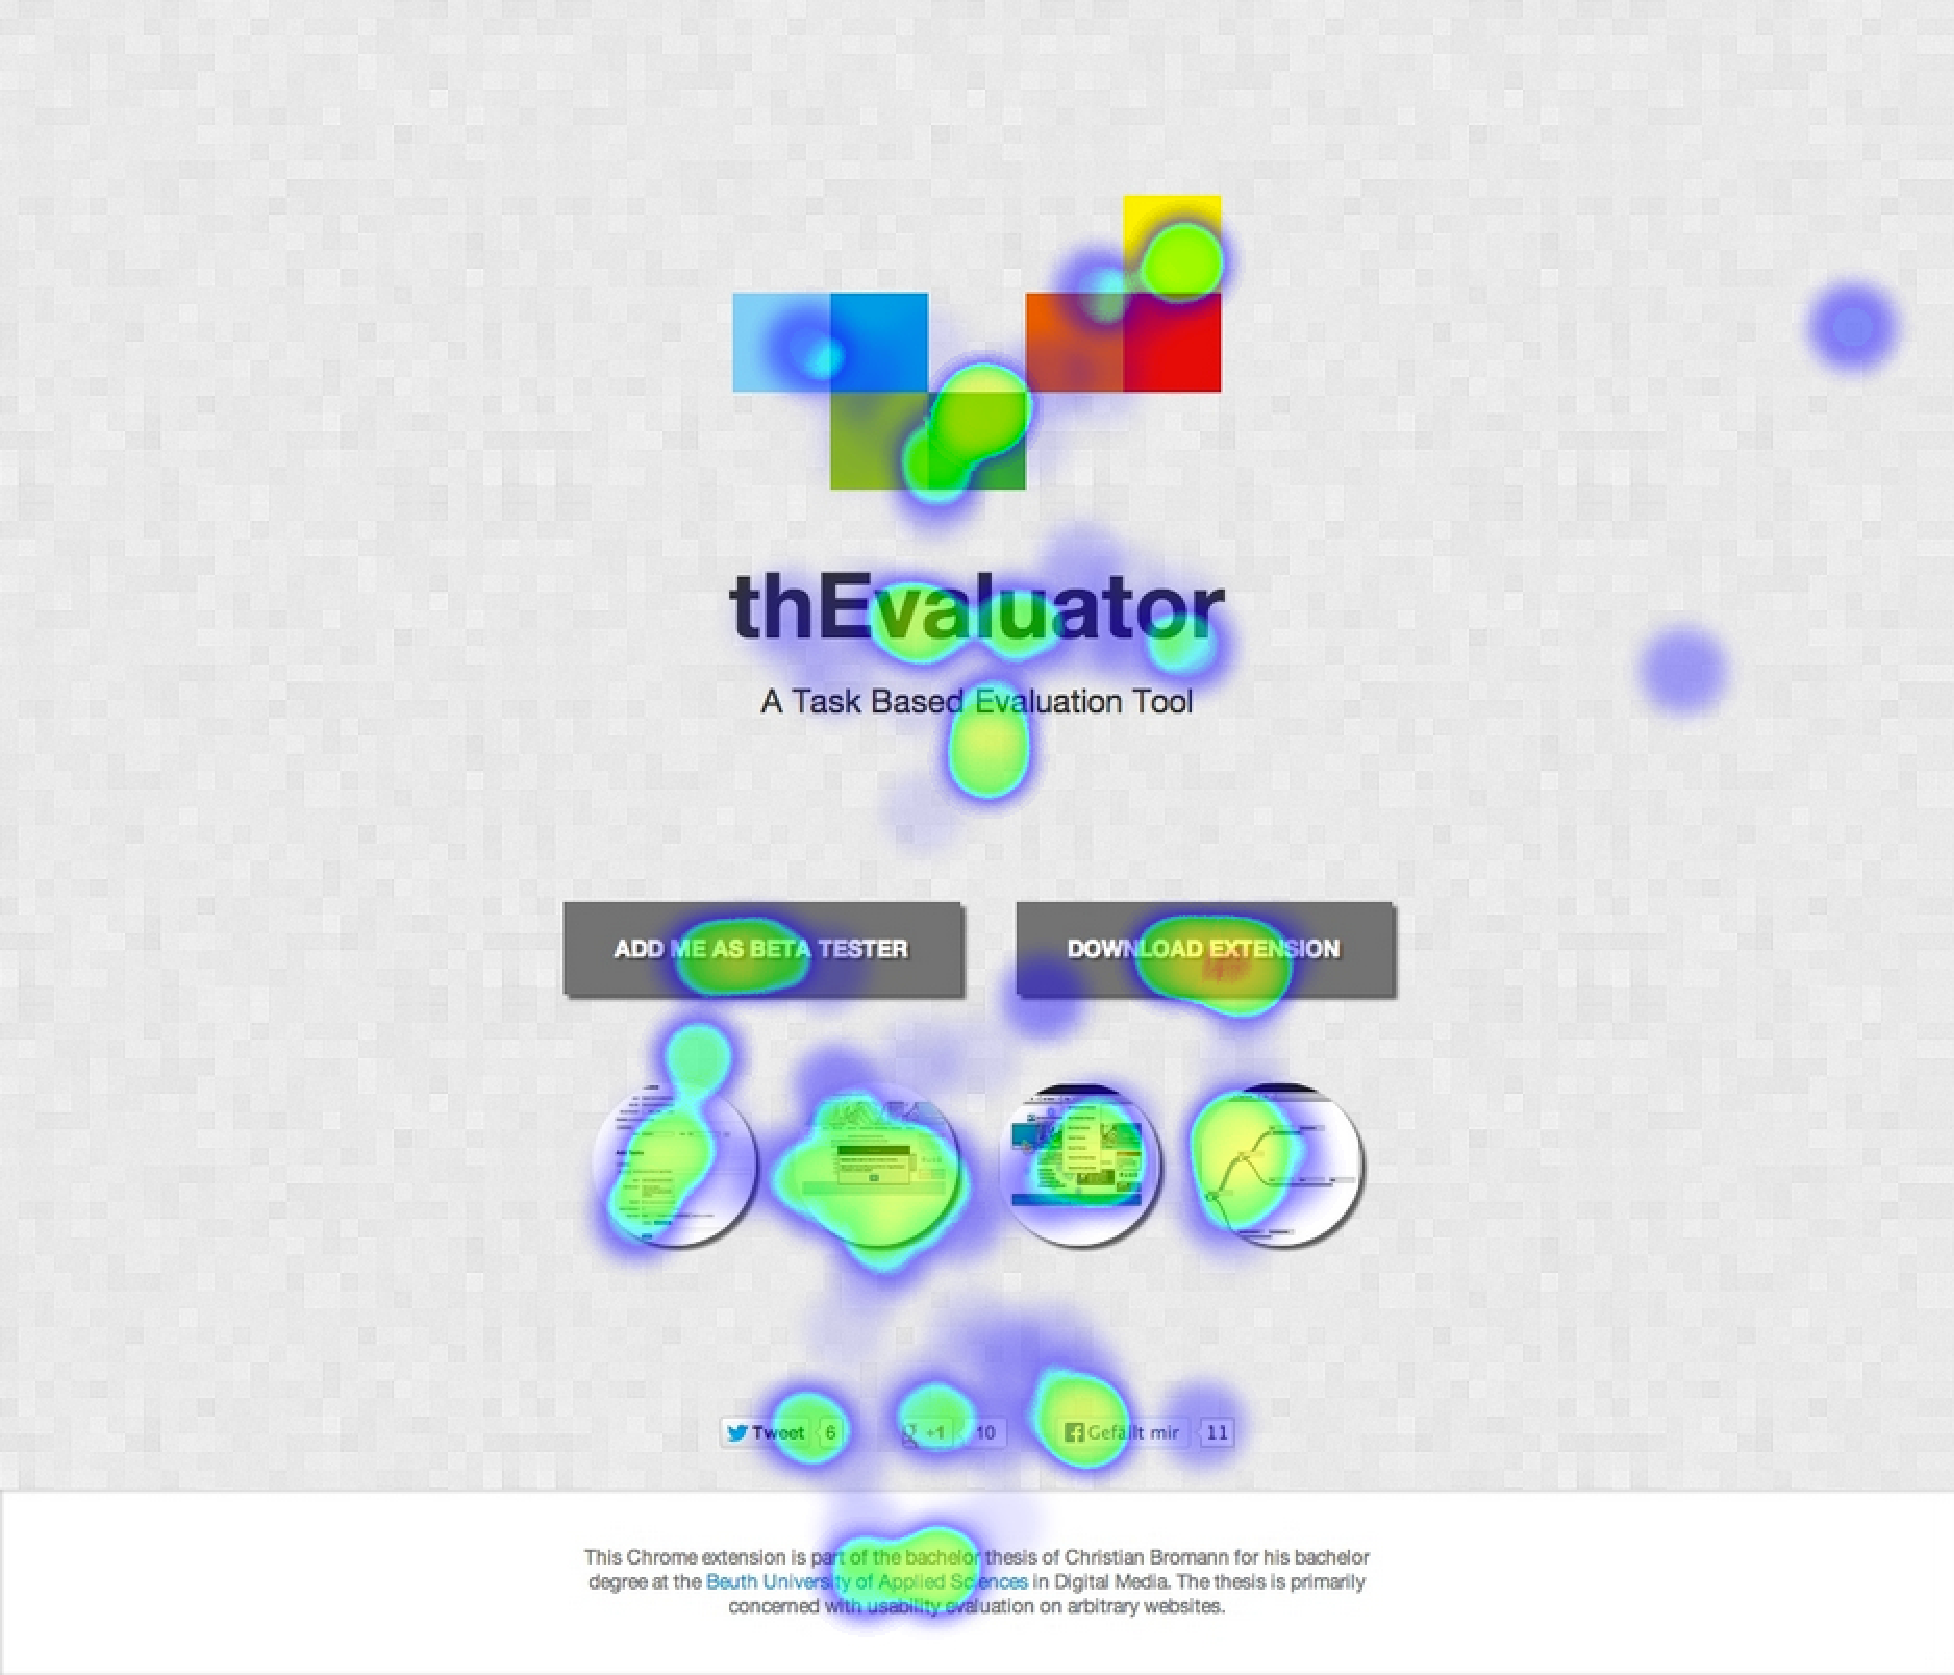
\includegraphics[scale=0.35]{./images/gazespot}
\end{center}
\begin{figure}[htb]
   \centering
   \caption{Beispiel einer Gazespot Visualisierung der \textit{thEvaluator} Projektwebsite}
    \label{gazespot}
\end{figure}


\subsection{Gazeplots}

Gazeplots konzentrieren sich ebenfalls auf Fixpunkte. Jedoch wird diesmal nicht durch Farbe ausgedrückt, wo die stärksten \Gls{Fixationen} auftreten, sondern durch nummerierte Kreise. Sie repräsentieren die Fixationsdauer. In den Kreisen steht eine numerische Zahl, die die Reihenfolge der Fixation angibt. Dadurch fließt eine zeitliche Dimension in die Auswertung mit ein. Linien verbinden letztendlich die Kreise und verdeutlichen somit den Bewegungsablauf der Maus. Dies wird auch als Sakkade bezeichnet.

\vspace{0.3cm}
\begin{center}
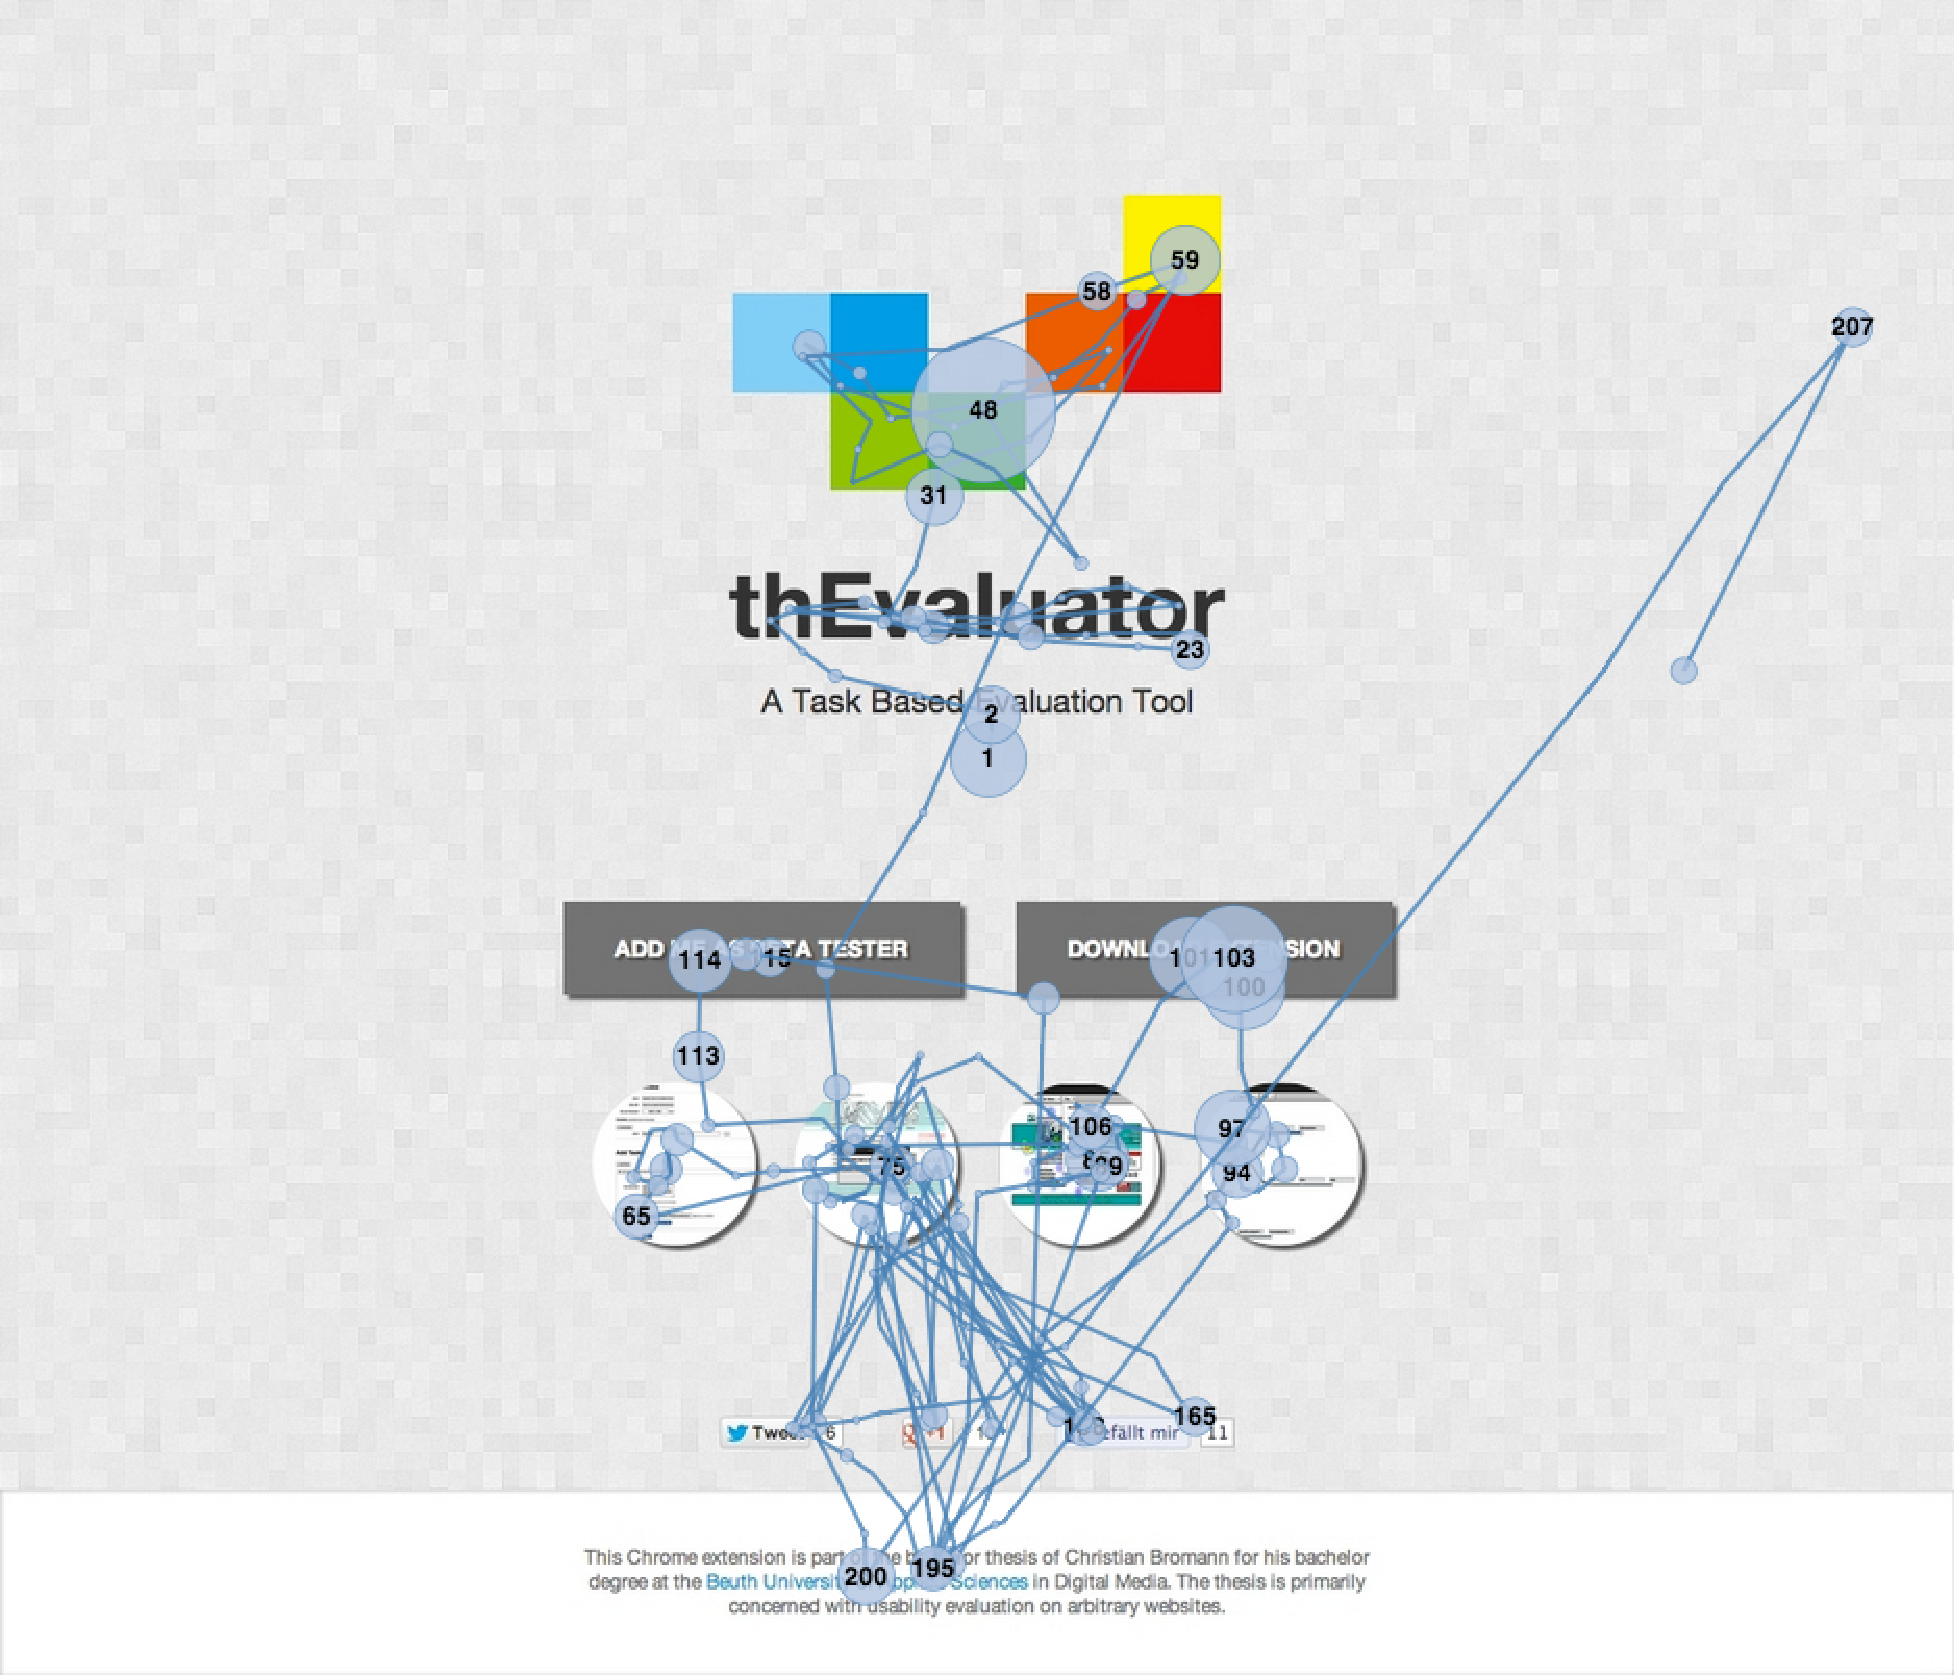
\includegraphics[scale=0.35]{./images/gazeplot}
\end{center}
\begin{figure}[htb]
   \centering
   \caption{Beispiel einer Gazeplot Visualisierung der \textit{thEvaluator} Projektwebsite}
    \label{gazeplot}
\end{figure}


\subsection{Attention-Maps}

Webseiten tendieren dazu, in der vertikalen Achse länger zu sein, als in der horizontalen. Dies liegt daran, dass das vertikale Scrollen viel natürlicher wirkt als das horizontale. Einen Nachteil haben trotzdem beide Arten. Die Wahrnehmung des Users sinkt, je weiter er scrollen muss. Wichtige Inhalte sollten daher immer direkt zu sehen sein. Dieser Usability Faktor kann ebenfalls durch eine Methode analysiert werden. Durch Attention-Maps (auch Scroll-Maps genannt) werden wieder über Farbverläufe Bereiche gekennzeichnet, die die meiste Aufmerksamkeit beim User erlangen. Inhalte, die durch den Bildschirm erfasst wurden, erhalten eine warme Farbe, hingegen Bereiche, zu denen der User gar nicht gekommen ist, da er nicht so weit gescrollt hat, eine kältere. Je nach Seitentyp ergibt dies meist ein einheitliches Muster. Die oberen Inhalte einer Seite werden immer rot gekennzeichnet. Je länger die Seite dann wird, desto kälter verläuft der Farbverlauf. Die Analyse über Attention Maps zeigt auf, ob eine Seite gekürzt werden muss oder nicht.\\
\\
Die Aufmerksamkeitsspanne beim Scrollen ist dabei stark abhängig vom Benutzertyp. Je nach Art der Seite verlieren User schneller oder langsamer die Lust daran. Bei Online-Shops stört dies beispielsweise nicht. Der Besucher stöbert hier gern durch lange Seiten und fühlt sich sogar beim Surfen gestört, wenn er schon nach kurzer Zeit eine neue Seite öffnen muss, um neue Produkte zu sehen. Oft findet man hier auch die Technik des \textit{Infinite Scrolling} wieder. Dabei werden Inhalte automatisch nachgeladen, sobald der User ans Ende der Seite gelangt. Dadurch wird ein Gefühl suggeriert, die Seite würde nie enden. Da der Besucher dabei die Inhalte schnell erforschen will, stört es ihn nicht, dass er dafür scrollen muss. Die Aufmerksamkeit bleibt nahezu konstant. Weitere Seiten, bei denen dies der Fall ist, sind Social Networks, Blogs oder Portfolio Seiten.\\
\\
Ganz anders hingegen ist es bei informationsbasierten Seiten mit viel mehr Text als Bild. Hier sucht der Nutzer nach bestimmten Informationen und hat weder Zeit noch Lust lange auf einer Seite nach diesen zu suchen. Das Vertrauen in die Qualität der Inhalte nimmt umso mehr ab, je länger er dafür auf der Seite suchen oder scrollen muss.